
\documentclass[../Main.tex]{subfiles}
\usepackage{makecell}
\begin{document}
Based on the real-world problems discussed in Chapter \ref{chapter:Introduction}, Chapter \ref{chapter:Related_works} aims to delve deeper into the existing products and solutions that can help address these issues. Specifically, it will also analyze some detailed use cases of the EPD display system, as outlined in Section \ref{section:2.2}.

\section{Status survey}
\label{section:2.1}
There are several e-paper display manufacturers that take advantage of EPD technology to provide solutions to multiple different businesses. This section will focus on four leading e-paper display providers: \textbf{E Ink}, \textbf{Seekink}, \textbf{Inkcase}, and \textbf{Pervasive Displays}.

\textbf{E Ink} is a leader in electronic paper (e-paper) display technology, co-founded in 1997 by MIT undergraduates and a professor from the MIT Media Lab. They offer a variety of e-paper display modules suited for diverse applications. Their products are used in several sectors, including reading and writing, education, business and office, mobile and wearables, retail, logistics and factories, healthcare, transportation, automotive, and innovative design. They also showcase customer-specific applications and provide optimized solutions and system integration for businesses. Although they have quality products and solutions aimed at a broad customer segment spread across various fields, E Ink focuses only on core e-paper technology with a few essential products such as eReaders, electronic shelf labels, and other low-power display needs. While beneficial for brand recognition and expertise in a specific area, this specialization can limit market reach and diversification compared to companies with a broader product range. Also, the manufacturing process for E Ink displays is complex and costly, which can lead to higher product prices, impacting competitiveness, especially in price-sensitive markets. That's why E Ink's specialized technology might not be as widely recognized or preferred by the average consumer in many specific regions, including Vietnam.

\textbf{Seekink} is recognized as a leading electronic paper display (EPD) manufacturer with eight years of experience. Seekink operates its automatic manufacturing base, which is capable of mass production, and emphasizes a high level of customization to meet diverse needs across markets. However, Seekink is not widely recognized in Vietnam, primarily because their marketing and sales strategies are focused on large enterprises. This focus on big businesses typically involves offering high-priced, specialized products and services that might not cater to the broader consumer market or smaller businesses. This approach can limit their market presence and brand recognition among the general public and smaller enterprises. 

\textbf{InkCase} is a product line from the Singapore-based consumer electronics design house Gajah. They specialize in offering protective cases for smartphones with added functionalities and are also involved in various innovative display solutions, including intelligent information display, healthcare, and tracking. 

\textbf{Pervasive Displays} is a leading manufacturer in the electronic paper display (EPD) industry, specializing in the design, manufacture, and marketing of e-paper displays. They have a manufacturing capacity of over 2 million pieces per week and are financially stable, being a part of the world's largest display company. Their products and services are tailored to industrial applications, with a focus on the design and manufacturing of ultra-low power displays, and are often ordered in large quantities by other major industrial clients.

With the assessments mentioned above, the features of the four e-paper display manufacturers can be summarized in the table \ref{fig:table_manufaturers} below.

\begin{table}[H]
    \renewcommand{\arraystretch}{2.5} % Adjust for row height
    \centering{}
    \fontsize{9pt}{8pt}\selectfont 
    \begin{tabular}{| m{2.0cm} | m{2.8cm} | m{2.8cm} | m{2.8cm} | m{2.8cm} |}
        \hline
        \textbf{Features}           & \textbf{E Ink}            & \textbf{Seekink}  & \textbf{InkCase} & \textbf{Pervasive Displays} \\ \hline
        \textbf{Prices}             & Contact sale              & Contact sale     & Not available & Contact sale                \\ \hline
        \textbf{Client type}        & \makecell[{{p{2.5cm}}}]{\raggedright Business\\Commercial user} & Business   & Commercial user & \Gape[10pt][-80pt]{\makecell[{{p{2.5cm}}}]{\raggedright Business\\Commercial user}}   \\ \hline
        \textbf{Use case}        & \Gape[10pt][-10pt]{\makecell[{{p{2cm}}}]{\raggedright Business\\Education\\Healthcare\\Logistics\\Transportation\\Automotive}} & \Gape[10pt][-10pt]{\makecell[{{p{2cm}}}]{\raggedright Business\\Retail\\Education\\Transportation\\Healthcare\\IoT}}  & \makecell[{{p{2cm}}}]{\raggedright Transportation\\Business} & \Gape[00pt][-20pt]{\makecell[{{p{2cm}}}]{\raggedright Logistic\\IoT\\Healthcare\\Education\\Business}}   \\ \hline
        \textbf{Management System}  & \checkmark & \checkmark & \checkmark & \checkmark \\ \hline
        \textbf{Allow custom display}  & Customized for each customer & Customized for each customer & Not available & Customized for each customer \\ \hline
        \textbf{Connectivities}     & \Gape[10pt][-10pt]{\makecell[{{p{2cm}}}]{\raggedright Bluetooth\\Internet\\Wired}} & \makecell[{{p{5cm}}}]{\raggedright Bluetooth\\Internet\\Wired}  & \makecell[{{p{5cm}}}]{\raggedright Bluetooth\\Internet} & Not published  \\ \hline
        \textbf{Other Products}     & Commercial e-paper electronic devices & E-paper display modules and devices  & E-paper protective phone cases & E-paper display modules and devices  \\ \hline
        \textbf{Available in Vietnam}        &   \scalebox{0.85}[1]{$\times$}       &   \scalebox{0.85}[1]{$\times$}                    & \scalebox{0.85}[1]{$\times$} & \scalebox{0.85}[1]{$\times$}        \\ \hline
    \end{tabular}
    \caption{Comparison table of four EPD manufacturers in e-paper display solutions}
    \label{fig:table_manufaturers}
\end{table}

Having learned from the survey of the above four systems and other real-life use cases, this project has concluded some objectives of building an EPD display system, including designing and building EPD devices, as well as including some essential features fitting in multiple use cases.

First, take the advantage of the electrophoretic display technology in displaying infromation. With the unique characteristic of e-paper disolay, the EPD device should be capable of displaying data for a long period of time without frequent refreshing. The device also need to be energy-saving and able to operate in reasonable time without recharging.

Second, manage EPD devices in a system via a central hub, which can be a cloud server, communicating with EPD devices and backend server using MQTT protocol and other wireless connectivities, or a local dock that is responsible for receiving data and displaying on EPD panels. Each solution's advantages and drawbacks are discussed in section \ref{section:optimization} in chapter \ref{chapter:SolutionAndContribution}.

Third, implement the EPD device system in some initial use cases to test the performance and effectiveness of the system in solving real-life problems. The initial use cases include name tags for students, employees, and clients; price tags in mini-markets and logistics services; and room and other signages.
  
Finally, implement security in the system and enhance user experience.

\section{Functional Overview}
\label{section:2.2}

\subsection{General use case diagram}
\label{subsection:2.2.1}
The general use case diagram of the EPD Display System is illustrated in Figure \ref{fig:uc_general}. As per the diagram, the system involves three main actors: The Manager, The Administrator, and the EPD devices. The Manager can manage EPD devices, data, and their accounts. The Administrator inherits the functions of the Manager and can also manage and test the devices more advanced. On the other hand, the EPD devices act as end-users, receiving and displaying data on the screen. They also interact with the system via the MQTT protocol.
\begin{figure}[htbp]
    \centering
    \begin{tikzpicture}
        % Define system boundary
        \umlactor[x=0, y=0]{Administrator}
        \umlactor[x=0, y=-4]{Manager}ssss
        \umlactor[x=11.5, y=0]{EPD Devices}
        
        \begin{umlsystem}[x=4, y=0]{System}
            % Define the use cases
            \umlusecase[x=2, y=0, name=usecase1, fill = white]{Account Management}
            \umlusecase[x=2, y=-2, name=usecase2, fill = white]{Device Management}
            \umlusecase[x=2, y=-4, name=usecase3, fill = white]{Data Management}
        \end{umlsystem}
        
        % Draw associations
        \umlassoc{Administrator}{usecase1}
        \umlassoc{Administrator}{usecase2}
        \umlassoc{Manager}{usecase2}
        \umlassoc{Manager}{usecase3}
        \umlassoc{Manager}{usecase1}
        \umlassoc{EPD Devices}{usecase1}
        \umlinherit{Administrator}{Manager} 
        
        \draw (-1.5, 2.5) rectangle (13, -6);
    \end{tikzpicture}
    \caption{General use case diagram of the EPD display system}
    \label{fig:uc_general}
\end{figure}

\subsection{Detailed use case diagram}
\label{subsection:2.2.2}

\subsubsection{Detailed use case of User's Account Management function}

Figure \ref{fig:uc_user} below describes the detailed use case diagram of the User's Account Management function, including the Manager and Administrator. Users can create a new account, log in, and modify personal information.

\begin{figure}[H]
    \centering
    \begin{tikzpicture}
        \umlactor[x=0, y=0]{Administrator}
        \umlactor[x=0, y=-4]{Manager}
    
        \begin{umlsystem}[x=4, y=0]{System}
            % Define the use cases
            \umlusecase[x=2, y=0, name=usecase1, fill = white]{Register}
            \umlusecase[x=2, y=-2, name=usecase2, fill = white]{Log in}
            \umlusecase[x=2, y=-4, width=3cm, name=usecase3, fill = white]{Manage personal information}
        \end{umlsystem}
        
        % Draw associations
        \umlassoc{Manager}{usecase1}
        \umlassoc{Manager}{usecase2}
        \umlassoc{Manager}{usecase3}
        \umlinherit{Administrator}{Manager} 
        
        \draw (-1.5, 2.5) rectangle (13, -6);
    \end{tikzpicture}
    \caption{Detailed use case of User's Account Management function}
    \label{fig:uc_user}
\end{figure}

\subsubsection{Detailed use case of Data Management function}
A detailed use case diagram of the Data Management function of the Manager is displayed in figure \ref{fig:uc_data}. This function enables the Manager to view, add, modify, remove data, and choose whether or not to display it on the EPD devices.

\begin{figure}[H]
    \centering
    \begin{tikzpicture}
        \umlactor[x=0, y=-2]{Manager}
        \umlactor[x=11.5, y=-2]{EPD Devices}
        
        \begin{umlsystem}[x=4, y=0]{System}
            % Define the use cases
            \umlusecase[x=0, y=0, name=usecase0, fill = white]{Add displaying data}
            \umlusecase[x=2, y=-1.5, width=3cm, name=usecase1, fill = white]{View the list of data}
            \umlusecase[x=1, y=-3, name=usecase2, fill = white]{Modify data}
            \umlusecase[x=2.5, y=-4.7, width=3cm, name=usecase3, fill = white]{Display data on device}
            \umlusecase[x=0, y=-6, name=usecase4, fill = white]{Remove data}
        \end{umlsystem}
        
        % Draw associations
        \umlassoc{Manager}{usecase0}
        \umlassoc{Manager}{usecase1}
        \umlassoc{Manager}{usecase2}
        \umlassoc{Manager}{usecase3}
        \umlassoc{Manager}{usecase4}
        \umlassoc{EPD Devices}{usecase2}
        \umlassoc{EPD Devices}{usecase3}
        
        \draw (-1.5, 2.5) rectangle (13, -8);
    \end{tikzpicture}
    \caption{Detailed use case of Data Management function}
    \label{fig:uc_data}
\end{figure}

\subsubsection{Detailed use case of Device Management function}
Figure \ref{fig:uc_device} illustrates the use case diagram of the Device Management function, showing two actors participating in the system. This function enables the Manager to view, add, modify, or remove device information. The Administrator, inheriting the functions of the Manager, can also debug the device after connecting it to the computer via a USB port. 

\begin{figure}[H]
    \centering
    \begin{tikzpicture}
        \umlactor[x=0, y=-2]{Manager}
        \umlactor[x=0, y=-6]{Administrator}
        \umlactor[x=11.5, y=-4]{EPD Devices}
        
        \begin{umlsystem}[x=4, y=0]{System}
            % Define the use cases
            \umlusecase[x=2, y=0, name=usecase1, fill = white]{View device list}
            \umlusecase[x=2, y=-2, width=3cm, name=usecase4, fill = white]{Modify device}
            \umlusecase[x=2, y=-3.5, name=usecase2, fill = white]{Add new device}
            \umlusecase[x=1.5, y=-5.3, width=3cm, name=usecase3, fill = white]{Remove device}
            \umlusecase[x=1, y=-7, width=3cm, name=usecase5, fill = white]{Debug, manage ESP}
        \end{umlsystem}
        % Draw associations
        \umlassoc{Manager}{usecase1}
        \umlassoc{Manager}{usecase2}
        \umlassoc{Manager}{usecase3}
        \umlassoc{Manager}{usecase4}
        \umlassoc{EPD Devices}{usecase1}
        \umlassoc{EPD Devices}{usecase2}
        \umlassoc{EPD Devices}{usecase3}
        \umlassoc{EPD Devices}{usecase4}
        \umlassoc{EPD Devices}{usecase5}
        \umlassoc{Administrator}{usecase5}
        \umlinherit{Administrator}{Manager} 
        
        \draw (-1.5, 2.5) rectangle (13, -9);
    \end{tikzpicture}
    \caption{Detailed use case of Device Management function}
    \label{fig:uc_device}
\end{figure}

\subsection{Business process}
\label{subsection:2.2.3}
The system comprises several business processes, with the most prominent ones being the process of adding data and displaying it on EPD devices and the process of adding EPD devices to the system. Each flow showcases how the system communicates with the device via USB and the MQTT protocol and how the device receives and processes data.

\subsubsection{"Creating new device" flow}
Figure \ref{fig:act_new-device} below shows the business process when the Manager creates and registers a new device to the system. This process requires the users to connect the EPD device to the computer via a USB port, choose from the list of connected devices, and then fill in the required information before submitting it to the system. Upon receipt of the submitted data, the system sends a data write request to the device via Serial Port. The EPD device then connects to the Internet with the received information and connects to the MQTT Broker before publishing its connection status to the system.

\begin{figure}[H]
    \centering
    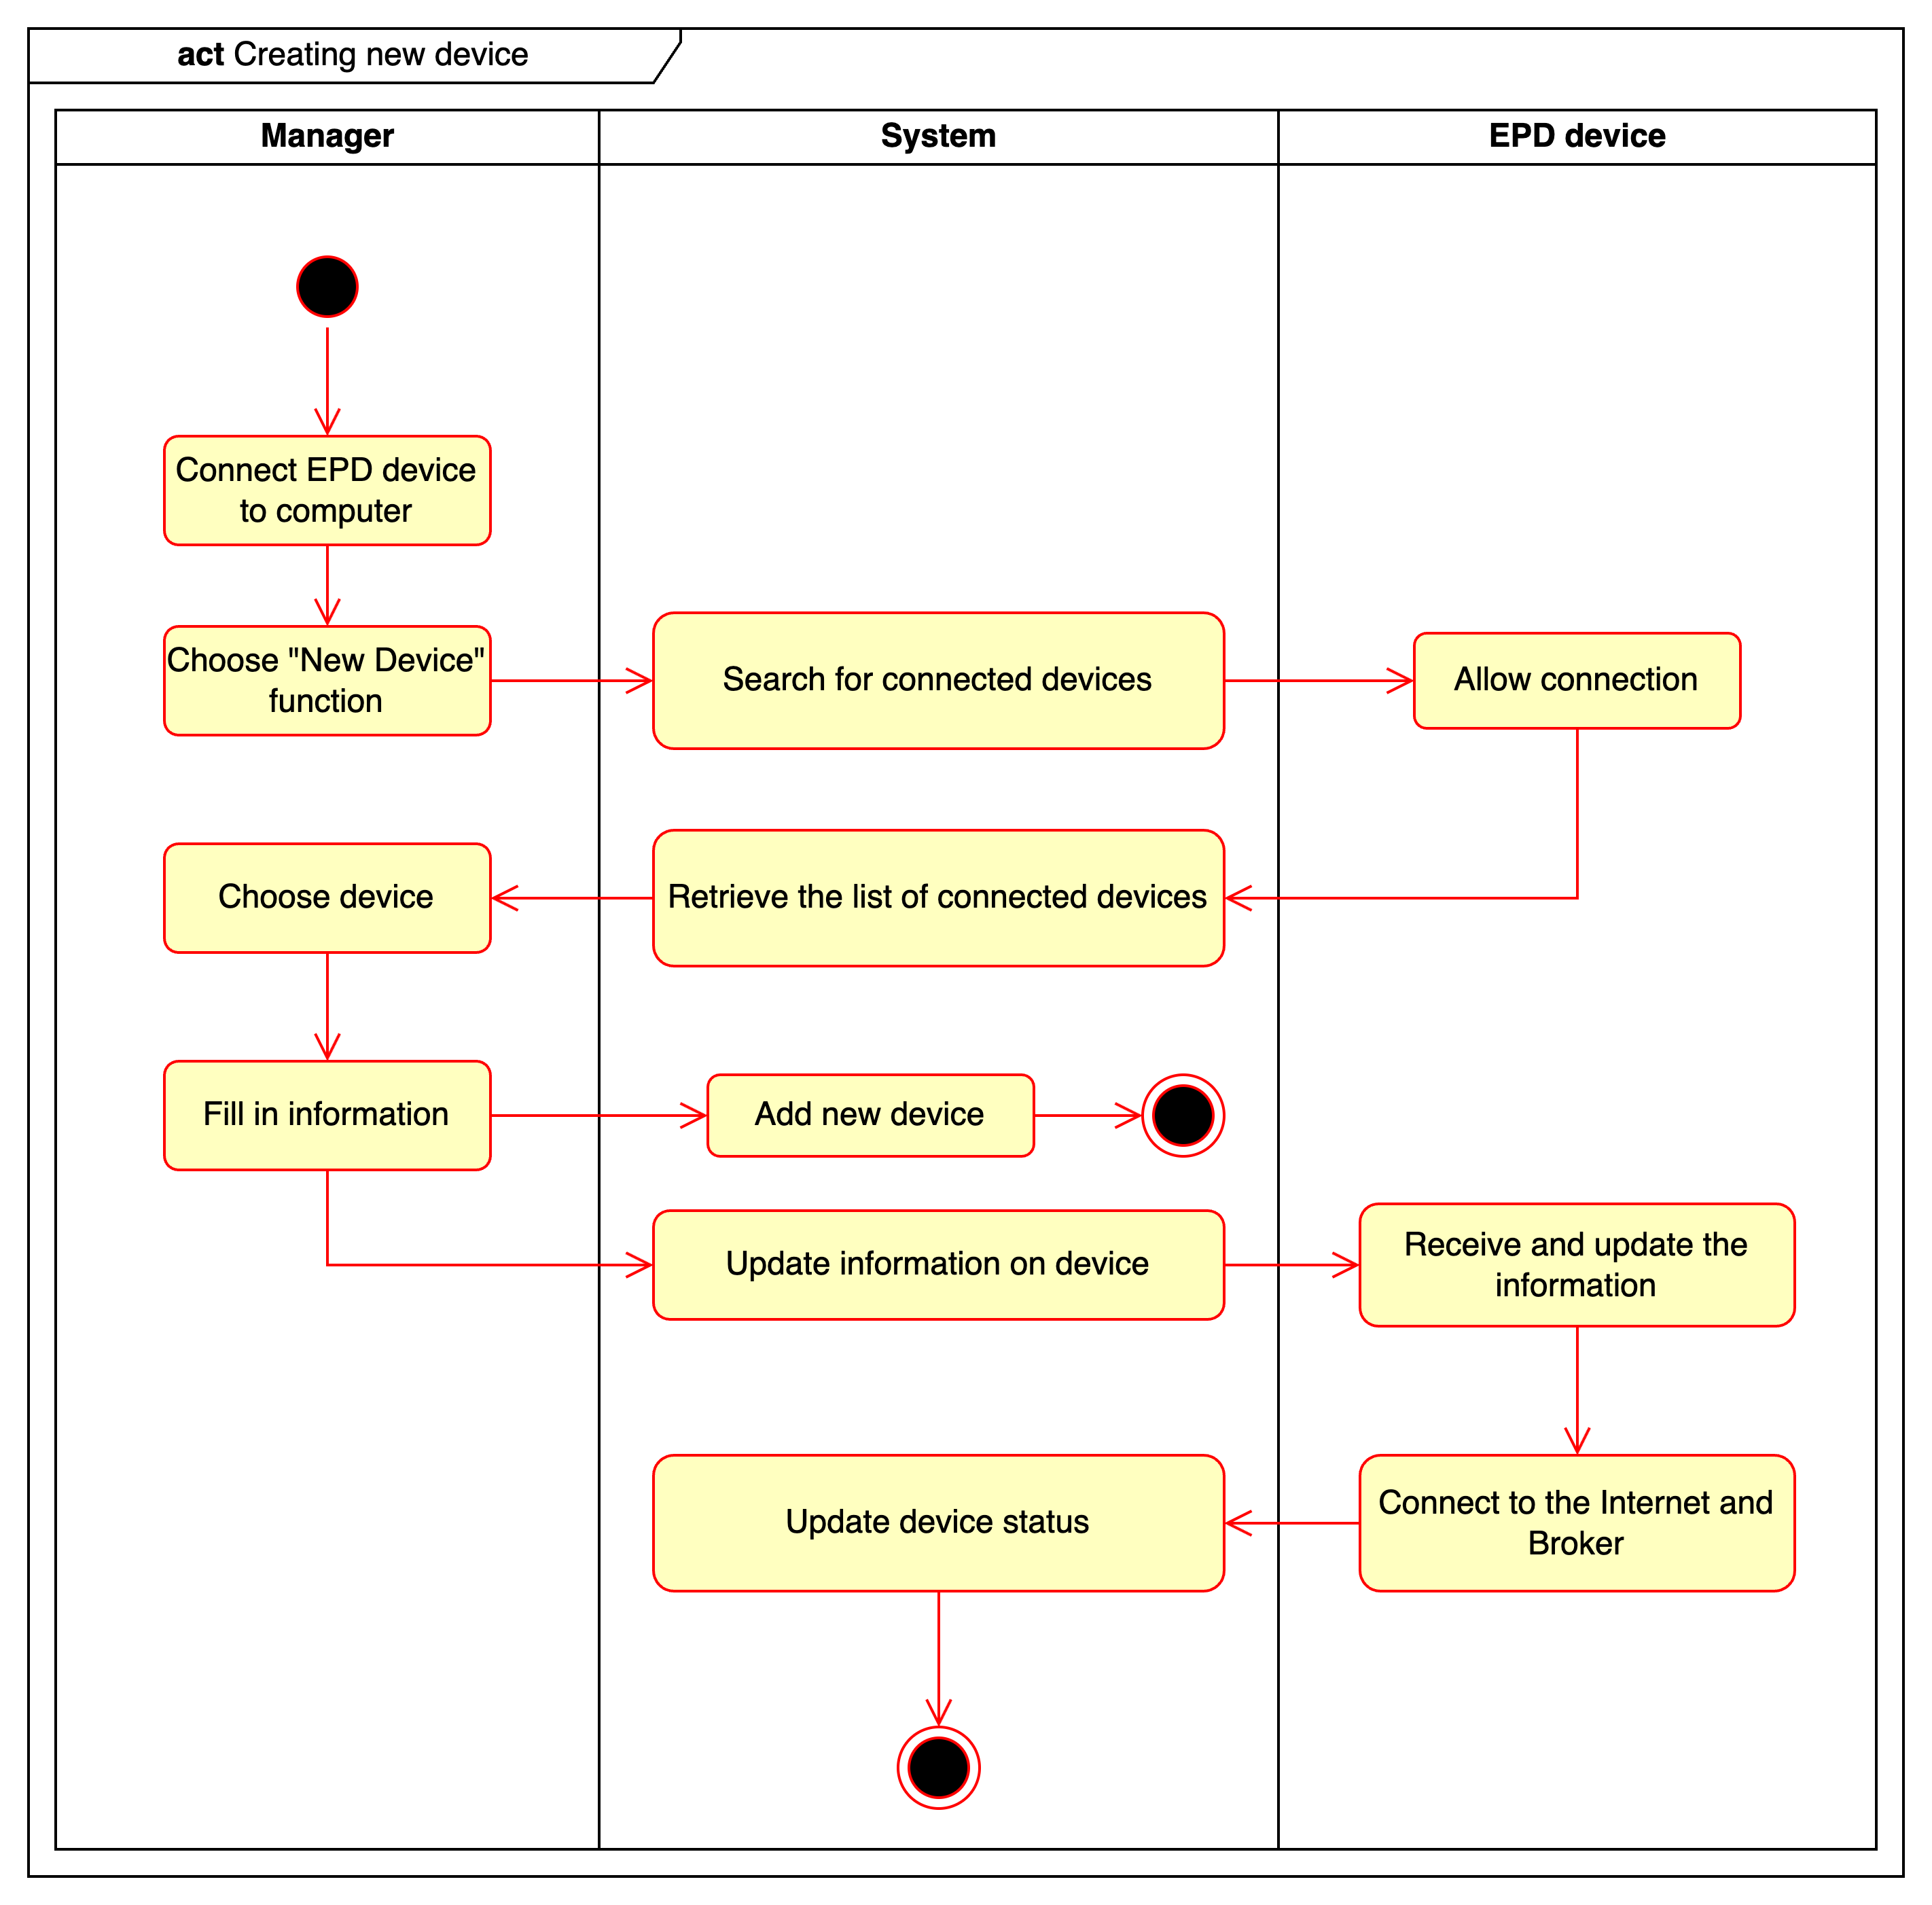
\includegraphics[scale=0.155]{doc/imgs/act_new-device.png}
    \caption{"Creating new device" business flow}
    \label{fig:act_new-device}
\end{figure}

\subsubsection{"Creating and displaying new data" flow}
The following describes the business process when users add new data to the system, as depicted in Figure \ref{fig:act_new-data}. Firstly, the user selects the type of data they want to display. Afterward, they add the corresponding detailed information based on the chosen data type. Users can also decide whether or not to allow display on the EPD device. If they choose to do so, the system will provide a list of devices connected to the MQTT Broker for the user to choose from. The user will then provide additional information about how to display the data on the selected device. Once all the necessary information has been provided, the system will send MQTT messages through the MQTT Broker. The selected device will receive and display the data and send the status back to the system via the MQTT protocol.

\begin{figure}[H]
    \centering
    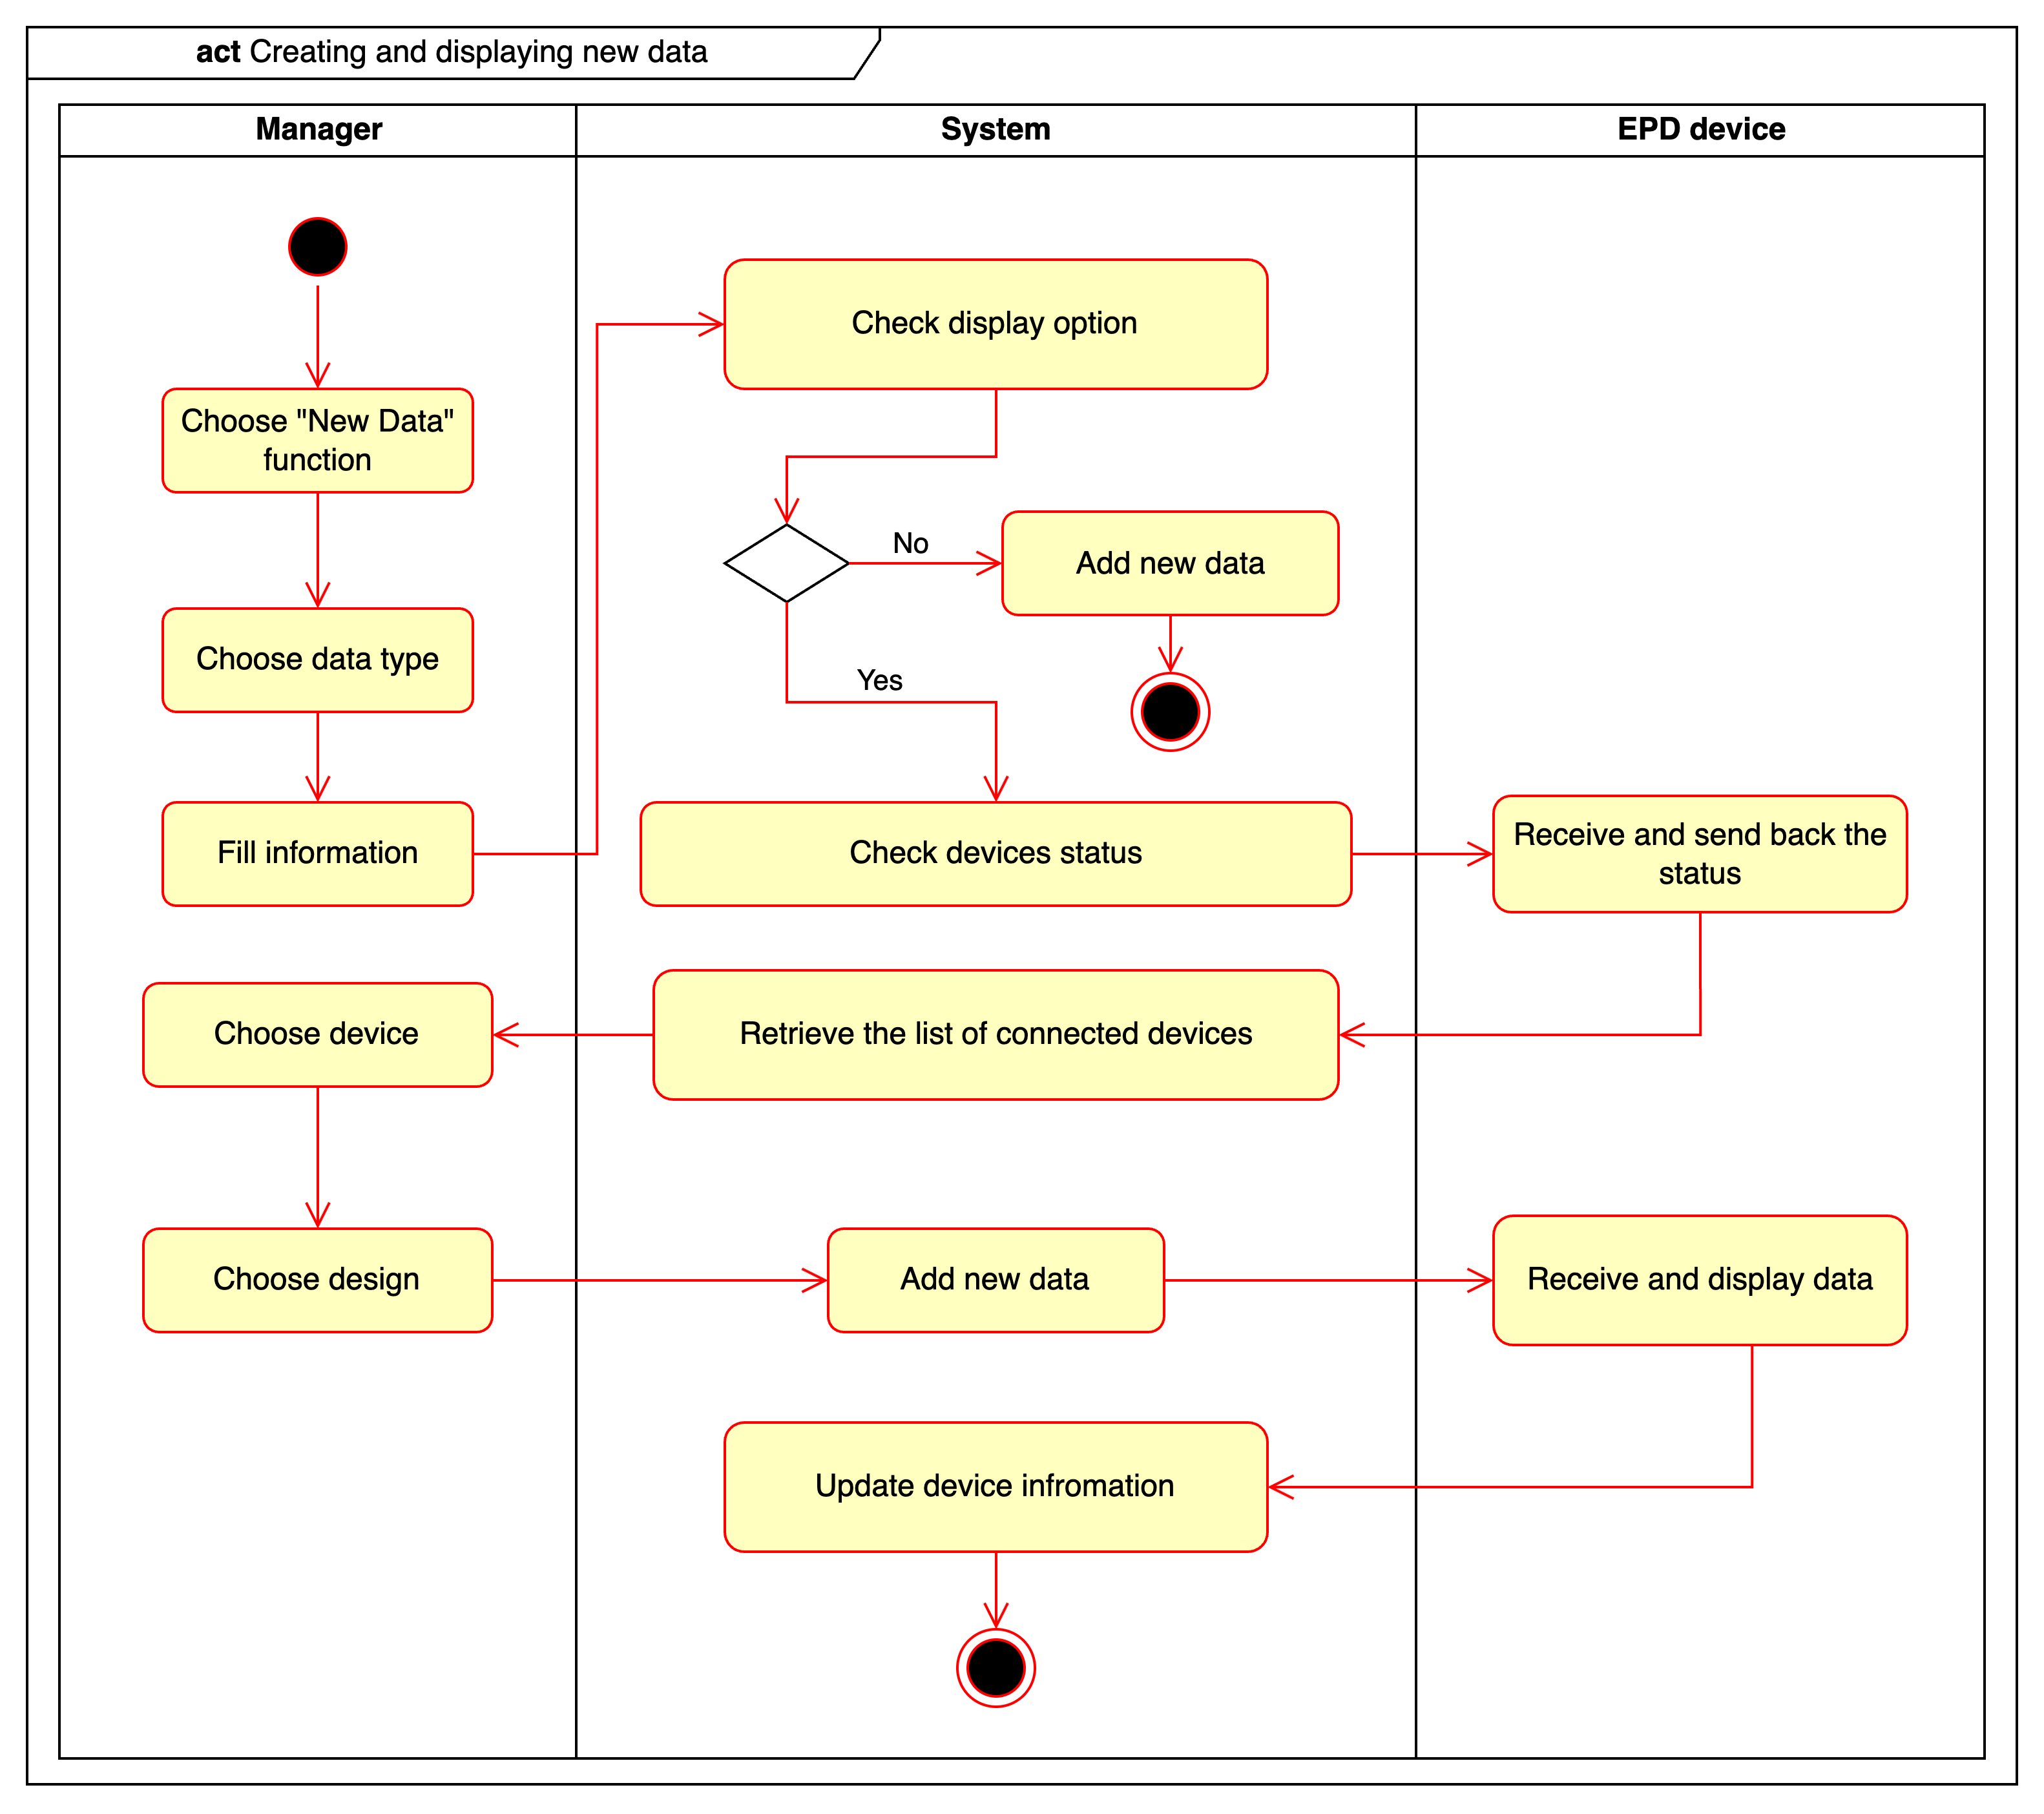
\includegraphics[scale=0.14]{doc/imgs/act_new-data.png}
    \caption{"Creating and displaying new data" business flow}
    \label{fig:act_new-data}
\end{figure}

\section{Functional description}
\label{section:2.3}
\begin{table}[H]
    \renewcommand{\arraystretch}{2} % Adjust for row height
    \centering{}
    \fontsize{9pt}{8pt}\selectfont 
    \begin{tabular}{| m{2cm} | m{4cm} |}
        \hline
        \textbf{ID} & \textbf{Name}             \\ \hline
        UC01        & Create new device         \\ \hline
        UC02        & Modify device information \\ \hline
        UC03        & Remove device             \\ \hline
        UC04        & Add new data              \\ \hline
        UC05        & Modify data information   \\ \hline
        UC06        & Remove data               \\ \hline
        UC07        & Create account            \\ \hline
        UC08        & Sign in                   \\ \hline
    \end{tabular}
    \caption{List of use cases}
    \label{fig:table_uc}
\end{table}

\subsection{Description of use case "Create new device"}
{\fontsize{9pt}{8pt}\selectfont 
    \newcolumntype{M}[1]{>{\centering\arraybackslash}m{#1}}
    \newcolumntype{L}[1]{>{\raggedright\arraybackslash}p{#1}}
    \renewcommand{\arraystretch}{2.5} % Adjust for row height
    \begin{longtable}{|L{2cm}|L{1cm}|L{2cm}|L{7cm}|}
        \hline
        \textbf{ID}             & UC01 & \textbf{Name} & Create new device \\ \hline
        \textbf{Actor}          & \multicolumn{3}{l|}{Manager, System, EPD device} \\ \hline
        \textbf{Pre-condition}  & \multicolumn{3}{p{12cm}|}{The user logs into the system as a Manager. To create a new device and edit device information in case the device is not connected to the Internet, users need to connect the device to the computer via a USB port.} \\ \hline
        
        \multirow{0}{2cm}{\textbf{Main scenario (success)}} & 
        \textbf{No.} & \textbf{Executed by} & \textbf{Action} \\ \cline{2-4}
        \endfirsthead
        \hline
        \multirow{0}{2cm}{\textbf{Main scenario (success)}} & 
        \textbf{No.} & \textbf{Executed by} & \textbf{Action} \\ \cline{2-4}
        \endhead
        & 1     & Manager               & Select "New Device" function\\ \cline{2-4}
        & 2     & System                & Retrieve and display the list of devices connected via USB \\ \cline{2-4}
        & 3     & Manager               & Choose a device from the list \\ \cline{2-4}
        & 4	    & System                & Connect to the device via Serial Port \\ \cline{2-4}
        & 5	    & System	            & Display the interface to enter device information \\ \cline{2-4}
        & 6     & Manager	            & Fill in the device information \textit{(described below *)} \\ \cline{2-4}
        & 7     & Manager	            & Send a request to create a new device \\ \cline{2-4}
        & 8	    & System	            & Store device information at the server and transmit data to the connected device \\ \cline{2-4}
        & 8.1	& System	            & Store device information at the server \\ \cline{2-4}
        & 8.2	& System	            & Transmit data to the EPD device \\ \cline{2-4}
        & 8.2.1	& Connected EPD device  & Process the received information \\ \cline{2-4}
        & 8.2.2	& Connected EPD device  & Connect to the Internet and MQTT Broker \\ \cline{2-4}
        & 8.2.3	& Connected EPD device	& Send status information to the server \\ \cline{2-4}
        & 8.2.4	& System	            & Receive and edit information of the new device \\ \cline{2-4}
        & 9	    & System	            & Notify successful device creation \\ \hline
    
        \multirow{0}{2cm}{\textbf{Extensions}} & 
        \textbf{No.} & \textbf{Executed by} & \textbf{Action} \\ \cline{2-4}
        & 4a.	 & System	& Error message: Unable to connect to the device\\ \cline{2-4}
        & 8.1a	 & System	& Error message: Need to enter all required fields of the device if the Manager misses any\\ \cline{2-4}
        & 8.2.2a & System	& If no update response is received from the device, save the device information\\ \hline

        \textbf{Post-condition}  & \multicolumn{3}{p{12cm}|}{The system store new device information in database} \\ \hline
    \end{longtable}
}

\subsection{Description of use case "Modify device information"}
{\fontsize{9pt}{8pt}\selectfont 
    \newcolumntype{M}[1]{>{\centering\arraybackslash}m{#1}}
    \newcolumntype{L}[1]{>{\raggedright\arraybackslash}p{#1}}
    \renewcommand{\arraystretch}{2.5} % Adjust for row height
    \begin{longtable}{|L{2cm}|L{1cm}|L{2cm}|L{7cm}|}
        \hline
        \textbf{ID}             & UC02 & \textbf{Name} & Modify device information \\ \hline
        \textbf{Actor}          & \multicolumn{3}{l|}{Manager, System, EPD device} \\ \hline
        \textbf{Pre-condition}  & \multicolumn{3}{p{12cm}|}{The user logs into the system as a Manager, and the device is registered in the system. To modify a device not connected to the Internet, users need to connect the device to the computer via a USB port.} \\ \hline
        
        \multirow{0}{2cm}{\textbf{Main scenario (success)}} & 
        \textbf{No.} & \textbf{Executed by} & \textbf{Action} \\ \cline{2-4}

        & 1     & Manager               & Access Dashboard, select Device \\ \cline{2-4}
        & 2     & System                & Retrieve and display the list of registered devices \\ \cline{2-4}
        & 3     & Manager               & Choose a device from the list and select Edit \\ \cline{2-4}
        & 4     & System                & Check the status of the device \\ \cline{2-4}
        & 4.1   & System                & If the device is not connected to the system, display a message asking the user to connect the device via USB \\ \cline{2-4}
        & 4.2   & Manager               & Connect the device via USB and choose from the list of connected devices \\ \cline{2-4}
        & 5     & System                & Display the interface to enter device information \textit{(described below *)} \\ \cline{2-4}
        & 6     & Manager               & Fill in and send a request to change device information \\ \cline{2-4}
        & 7     & System                & Save the new updated information \\ \cline{2-4}
        & 7.1   & System                & If the device is connected via USB, transmit data to the connected EPD device \\ \cline{2-4}
        & 7.2   & System                & If the device is connected to the MQTT server, send a request to change information on the device via the MQTT protocol \\ \cline{2-4}
        & 8     & Connected EPD device  & Process the received information \\ \cline{2-4}
        & 8.1   & Connected EPD device  & If the device is connected via USB, connect to the Internet and MQTT Broker \\ \cline{2-4}
        & 9     & Connected EPD device  & Send status information to the server \\ \cline{2-4}
        & 10    & System                & Receive and edit information of the new device \\ \cline{2-4}
        & 11    & System                & Notify successful device information change \\ \hline

        \multirow{0}{2cm}{\textbf{Extensions}} & 
        \textbf{No.} & \textbf{Executed by} & \textbf{Action} \\ \cline{2-4}
        \endfirsthead
        \hline
        \multirow{0}{2cm}{\textbf{Extensions}} & 
        \textbf{No.} & \textbf{Executed by} & \textbf{Action} \\ \cline{2-4}
        \endhead
        & 4.2a.  & System    & Error message: Unable to connect to the device \\ \cline{2-4}
        & 7a.    & System    & Error message: Need to enter all required fields of the device if Manager misses any \\ \cline{2-4}
        & 10a.   & System    & If no update response is received from the device, save the device information \\ \hline

        \textbf{Post-condition}  & \multicolumn{3}{p{12cm}|}{The system store new device updated information in database} \\ \hline
    \end{longtable}
}

\subsection{Description of use case "Remove a device"}
{\fontsize{9pt}{8pt}\selectfont 
    \newcolumntype{M}[1]{>{\centering\arraybackslash}m{#1}}
    \newcolumntype{L}[1]{>{\raggedright\arraybackslash}p{#1}}
    \renewcommand{\arraystretch}{2.5} % Adjust for row height
    \begin{longtable}{|L{2cm}|L{1cm}|L{2cm}|L{7cm}|}
        \hline
        \textbf{ID}             & UC03 & \textbf{Name} & Remove a device \\ \hline
        \textbf{Actor}          & \multicolumn{3}{l|}{Manager, System, EPD device} \\ \hline
        \textbf{Pre-condition}  & \multicolumn{3}{p{12cm}|}{The user logs into the system as a Manager, and the device is registered in the system.} \\ \hline
        
        \multirow{0}{2cm}{\textbf{Main scenario (success)}} & 
        \textbf{No.} & \textbf{Executed by} & \textbf{Action} \\ \cline{2-4}
        \endfirsthead
        \hline
        \multirow{0}{2cm}{\textbf{Main scenario (success)}} & 
        \textbf{No.} & \textbf{Executed by} & \textbf{Action} \\ \cline{2-4}
        \endhead
        & 1     & Manager       & Access the Dashboard, select Device \\ \cline{2-4}
        & 2     & System        & Retrieve and display the list of registered devices \\ \cline{2-4}
        & 3     & Manager       & Choose a device from the list and select Delete \\ \cline{2-4}
        & 4     & System        & Display a warning asking the user to confirm deletion \\ \cline{2-4}
        & 5     & Manager       & Confirm deletion of data \\ \cline{2-4}
        & 6     & System        & Check the display status of the device \\ \cline{2-4}
        & 6.1   & System        & If the device is not displaying data, remove the device from the system \\ \cline{2-4}
        & 6.2   & System        & If the device is displaying data, send a request to delete data on the device via MQTT \\ \cline{2-4}
        & 6.2.1 & EPD Device    & Process the received information, delete the displaying data information \\ \cline{2-4}
        & 6.2.3 & System        & Remove device display information from the data \\ \cline{2-4}
        & 7     & System        & Notify successful remove \\ \hline
    
        \multirow{0}{2cm}{\textbf{Extensions}} & 
        \textbf{No.} & \textbf{Executed by} & \textbf{Action} \\ \cline{2-4}
        & 6a.    & System               & End the use case if the user confirms not to delete the device \\ \cline{2-4}
        & 6.2.3a & System               & Error message: Unable to delete the device if an error occurs during deletion \\ \hline
        
        \textbf{Post-condition}  & \multicolumn{3}{p{12cm}|}{No} \\ \hline
    \end{longtable}
}

\subsection{Description of use case "Add new data"}
{\fontsize{9pt}{8pt}\selectfont 
    \newcolumntype{M}[1]{>{\centering\arraybackslash}m{#1}}
    \newcolumntype{L}[1]{>{\raggedright\arraybackslash}p{#1}}
    \renewcommand{\arraystretch}{2.5} % Adjust for row height
    \begin{longtable}{|L{2cm}|L{1cm}|L{2cm}|L{7cm}|}
        \hline
        \textbf{ID}             & UC04 & \textbf{Name} & Add new data \\ \hline
        \textbf{Actor}          & \multicolumn{3}{l|}{Manager, System, EPD device} \\ \hline
        \textbf{Pre-condition}  & \multicolumn{3}{p{12cm}|}{The user logs into the system as a Manager.} \\ \hline
        
        \multirow{0}{2cm}{\textbf{Main scenario (success)}} & 
        \textbf{No.} & \textbf{Executed by} & \textbf{Action} \\ \cline{2-4}
        \endfirsthead
        \hline
        \multirow{0}{2cm}{\textbf{Main scenario (success)}} & 
        \textbf{No.} & \textbf{Executed by} & \textbf{Action} \\ \cline{2-4}
        \endhead
        & 1     & Manager       & Select "New Data" function \\ \cline{2-4}
        & 2     & System        & Display the interface to choose data type to add \\ \cline{2-4}
        & 3     & Manager       & Choose the type of data from the list \\ \cline{2-4}
        & 4     & System        & Display the interface to enter data information \\ \cline{2-4}
        & 5     & Manager       & Fill in the data information \textit{(described below **)} \\ \cline{2-4}
        & 5.1   & System        & If the user chooses to display on a device, show the interface to select device and design \\ \cline{2-4}
        & 5.2   & Manager       & Choose device to display, and choose the design \\ \cline{2-4}
        & 6     & Manager       & Send a request to create new data \\ \cline{2-4}
        & 7     & System        & Save new data information on the server \\ \cline{2-4}
        & 7.1   & System        & If the user chooses to display data, transmit data to the connected EPD device \\ \cline{2-4}
        & 7.2   & EPD Device    & Process the received information \\ \cline{2-4}
        & 7.3   & EPD Device    & Display the data \\ \cline{2-4}
        & 7.4   & EPD Device    & Send status information to the server \\ \cline{2-4}
        & 7.5   & System        & Receive and update data information\\ \cline{2-4}
        & 8     & System        & Notify successful creation of the data \\ \hline
        
        \multirow{0}{2cm}{\textbf{Extensions}} & 
        \textbf{No.} & \textbf{Executed by} & \textbf{Action} \\ \cline{2-4}
        & 4a	& System        & Error: Need to enter all required fields of the device if the Manager misses any \\ \cline{2-4}
        & 5.1a  & System        & If there are no active devices, notify users and finish the use case \\ \cline{2-4}
        & 7.1a	& System	    & Error: Can't write data to the device \\ \hline
        
        \textbf{Post-condition}  & \multicolumn{3}{p{12cm}|}{The system store new data in database} \\ \hline
    \end{longtable}
}
\subsection{Description of use case "Modify data information"}
{\fontsize{9pt}{8pt}\selectfont 
    \newcolumntype{M}[1]{>{\centering\arraybackslash}m{#1}}
    \newcolumntype{L}[1]{>{\raggedright\arraybackslash}p{#1}}
    \renewcommand{\arraystretch}{2.5} % Adjust for row height
    \begin{longtable}{|L{2cm}|L{1cm}|L{2cm}|L{7cm}|}
        \hline
        \textbf{ID}             & UC05 & \textbf{Name} & Modify data information \\ \hline
        \textbf{Actor}          & \multicolumn{3}{l|}{Manager, System, EPD device} \\ \hline
        \textbf{Pre-condition}  & \multicolumn{3}{p{12cm}|}{The user logs into the system as a Manager, and the data is stored in the system.} \\ \hline
        
        \multirow{0}{2cm}{\textbf{Main scenario (success)}} & 
        \textbf{No.} & \textbf{Executed by} & \textbf{Action} \\ \cline{2-4}
        \endfirsthead
        \hline
        \multirow{0}{2cm}{\textbf{Main scenario (success)}} & 
        \textbf{No.} & \textbf{Executed by} & \textbf{Action} \\ \cline{2-4}
        \endhead
        & 1     & Manager       & Access Dashboard, select Data \\ \cline{2-4}
        & 2     & System        & Retrieve and display the list of data \\ \cline{2-4}
        & 3     & Manager       & Choose a data from the list and select Edit \\ \cline{2-4}
        & 4     & System        & Display the interface to enter data information \\ \cline{2-4}
        & 5     & Manager       & Fill in the data information \textit{(described below **)} \\ \cline{2-4}
        & 5.1   & System        & If the user chooses to display on a device, show the interface to select device and design \\ \cline{2-4}
        & 5.2   & Manager       & Choose device to display, and choose the design \\ \cline{2-4}
        & 6     & Manager       & Send a request to update data \\ \cline{2-4}
        & 7     & System        & Save the updated data on the server \\ \cline{2-4}
        & 7.1   & System        & If the user chooses to display data, transmit data to the connected EPD device \\ \cline{2-4}
        & 7.2   & EPD Device    & Process the received information \\ \cline{2-4}
        & 7.3   & EPD Device    & Display the data \\ \cline{2-4}
        & 7.4   & EPD Device    & Send status information to the server \\ \cline{2-4}
        & 7.5   & System        & Receive and update data information\\ \cline{2-4}
        & 8     & System        & Notify successful update \\ \hline
        
        \multirow{0}{2cm}{\textbf{Extensions}} & 
        \textbf{No.} & \textbf{Executed by} & \textbf{Action} \\ \cline{2-4}
        & 4a	& System    	& Error: Need to enter all required fields of the device if the Manager misses any \\ \cline{2-4}
        & 5.1a  & System        & If there are no active devices, notify users and finish the use case \\ \cline{2-4}
        & 7.1a	& System	    & Error: Can't write data to the device \\ \hline
        
        \textbf{Post-condition}  & \multicolumn{3}{p{12cm}|}{The system store new updated data in database} \\ \hline
    \end{longtable}
}

\subsection{Description of use case "Remove data"}
{\fontsize{9pt}{8pt}\selectfont 
    \newcolumntype{M}[1]{>{\centering\arraybackslash}m{#1}}
    \newcolumntype{L}[1]{>{\raggedright\arraybackslash}p{#1}}
    \renewcommand{\arraystretch}{2.5} % Adjust for row height
    \begin{longtable}{|L{2cm}|L{1cm}|L{2cm}|L{7cm}|}
        \hline
        \textbf{ID}             & UC06 & \textbf{Name} & Remove data \\ \hline
        \textbf{Actor}          & \multicolumn{3}{l|}{Manager, System, EPD device} \\ \hline
        \textbf{Pre-condition}  & \multicolumn{3}{p{12cm}|}{The user logs into the system as a Manager, and the data is stored in the system.} \\ \hline
        
        \hline
        \multirow{0}{2cm}{\textbf{Main scenario (success)}} & 
        \textbf{No.} & \textbf{Executed by} & \textbf{Action} \\ \cline{2-4}
        \endfirsthead
        \hline
        \multirow{0}{2cm}{\textbf{Main scenario (success)}} & 
        \textbf{No.} & \textbf{Executed by} & \textbf{Action} \\ \cline{2-4}
        \endhead
        & 1     & Manager       & Access Dashboard, select Data \\ \cline{2-4}
        & 2     & System        & Retrieve and display the list of data \\ \cline{2-4}
        & 3     & Manager       & Choose a data from the list and select Delete \\ \cline{2-4}
        & 4     & System        & Display a warning asking the user to confirm deletion \\ \cline{2-4}
        & 5     & Manager       & Confirm deletion of data \\ \cline{2-4}
        & 6     & System        & Check the display status of the data \\ \cline{2-4}
        & 6.1   & System        & If the data is being displayed, send a request to delete data on the device via MQTT \\ \cline{2-4}
        & 6.2   & EPD Device    & Process the received information, delete the displaying data information \\ \cline{2-4}
        & 6.3   & System        & Remove data information on the device \\ \cline{2-4}
        & 7     & System        & Remove the data from the system \\ \cline{2-4}
        & 8     & System        & Notify successful remove \\ \hline
        
        \multirow{0}{2cm}{\textbf{Extensions}} & 
        \textbf{No.} & \textbf{Executed by} & \textbf{Action} \\ \cline{2-4}
        & 6a    & System        & End the use case if the user confirms not to delete the data \\ \cline{2-4}
        & 7a    & System        & Error message: Unable to delete the device if an error occurs during deletion \\ \hline
        
        \textbf{Post-condition}  & \multicolumn{3}{p{12cm}|}{No} \\ \hline
    \end{longtable}
}

\subsection{Description of use case "Create account"}
{\fontsize{9pt}{8pt}\selectfont 
    \newcolumntype{M}[1]{>{\centering\arraybackslash}m{#1}}
    \newcolumntype{L}[1]{>{\raggedright\arraybackslash}p{#1}}
    \renewcommand{\arraystretch}{2.5} % Adjust for row height
    \begin{longtable}{|L{2cm}|L{1cm}|L{2cm}|L{7cm}|}
        \hline
        \textbf{ID}             & UC07 & \textbf{Name} & Create account \\ \hline
        \textbf{Actor}          & \multicolumn{3}{l|}{Manager, System} \\ \hline
        \textbf{Pre-condition}  & \multicolumn{3}{p{12cm}|}{No} \\ \hline
        
        \hline
        \multirow{0}{2cm}{\textbf{Main scenario (success)}} & 
        \textbf{No.} & \textbf{Executed by} & \textbf{Action} \\ \cline{2-4}
        \endfirsthead
        \hline
        \multirow{0}{2cm}{\textbf{Main scenario (success)}} & 
        \textbf{No.} & \textbf{Executed by} & \textbf{Action} \\ \cline{2-4}
        \endhead
        & 1     & Manager   & Go to the sign-up page \\ \cline{2-4}
        & 2     & System    & Display the interface to fill user information \\ \cline{2-4}
        & 3     & Manager   & Fill in the user information \textit{(described below ***)} \\ \cline{2-4}
        & 4     & Manager   & Send a request to create new account \\ \cline{2-4}
        & 5     & System    & Save new user information on the server \\ \cline{2-4}
        & 6     & System    & Notify successful creation of the user, and direct to log-in page \\ \hline
        
        \textbf{Extensions}  & \multicolumn{3}{p{12cm}|}{No} \\ \hline
        \textbf{Post-condition}  & \multicolumn{3}{p{12cm}|}{No} \\ \hline
    \end{longtable}
}

\subsection{Description of use case "Sign in"}
{\fontsize{9pt}{8pt}\selectfont 
    \newcolumntype{M}[1]{>{\centering\arraybackslash}m{#1}}
    \newcolumntype{L}[1]{>{\raggedright\arraybackslash}p{#1}}
    \renewcommand{\arraystretch}{2.5} % Adjust for row height
    \begin{longtable}{|L{2cm}|L{1cm}|L{2cm}|L{7cm}|}
        \hline
        \textbf{ID}             & UC08 & \textbf{Name} & Sign in \\ \hline
        \textbf{Actor}          & \multicolumn{3}{l|}{Manager, System} \\ \hline
        \textbf{Pre-condition}  & \multicolumn{3}{p{12cm}|}{The user have stored account.} \\ \hline
        
        \hline
        \multirow{0}{2cm}{\textbf{Main scenario (success)}} & 
        \textbf{No.} & \textbf{Executed by} & \textbf{Action} \\ \cline{2-4}
        \endfirsthead
        \hline
        \multirow{0}{2cm}{\textbf{Main scenario (success)}} & 
        \textbf{No.} & \textbf{Executed by} & \textbf{Action} \\ \cline{2-4}
        \endhead
        & 1     & Manager   & Go to the sign-in page \\ \cline{2-4}
        & 2     & System    & Display the interface to fill user email and password \\ \cline{2-4}
        & 3     & Manager   & Fill in the user credentials \\ \cline{2-4}
        & 4     & Manager   & Send a request to check account \\ \cline{2-4}
        & 5     & System    & Notify successful log-in, and redirect to dashboard page \\ \hline

        \multirow{0}{2cm}{\textbf{Extensions}} & 
        \textbf{No.} & \textbf{Executed by} & \textbf{Action} \\ \cline{2-4}
        & 5a    & System    & Error: User's credentials are incorrect \\ \hline
        
        \textbf{Post-condition}  & \multicolumn{3}{p{12cm}|}{No} \\ \hline
    \end{longtable}
}

(*) The input data of the device:
\begin{table}[H]
    \renewcommand{\arraystretch}{2} % Adjust for row height
    \centering{}
    \fontsize{9pt}{8pt}\selectfont 
    \begin{tabular}{| m{0.5cm} | m{2.5cm} | m{6cm} | m{2cm} |}
        \hline
        \textbf{No.}& \textbf{Name} & \textbf{Description}                          & \textbf{Required} \\ \hline
        1           & Name          & Name of the device                            & \checkmark        \\ \hline
        2           & SSID          & Name of the network the device connects to    & \checkmark        \\ \hline
        3           & Password      & Password of the network the device connects to& \checkmark        \\ \hline
    \end{tabular}
\end{table}

(**) The input data of data:
\begin{table}[H]
    \renewcommand{\arraystretch}{2} % Adjust for row height
    \centering{}
    \fontsize{9pt}{8pt}\selectfont 
    \begin{tabular}{| m{0.5cm} | m{2.5cm} | m{6cm} | m{2cm} |}
        \hline
        \textbf{No.}& \textbf{Name}     & \textbf{Description}                          & \textbf{Required}             \\ \hline
        1           & Type              & Type of the data                              & \checkmark                    \\ \hline
        2           & Name              & Name of the data                              & \checkmark                    \\ \hline
        3           & Email             & Email data, depend on data type               & \scalebox{0.85}[1]{$\times$}  \\ \hline
        4           & Student ID        & Student ID data, depend on data type          & \scalebox{0.85}[1]{$\times$}  \\ \hline
        5           & Class             & Class of the student, depend on data type     & \scalebox{0.85}[1]{$\times$}  \\ \hline
        6           & Employee ID       & Employee ID data, depend on data type         & \scalebox{0.85}[1]{$\times$}  \\ \hline
        7           & Department        & Department of employee, depend on data type   & \scalebox{0.85}[1]{$\times$}  \\ \hline
        8           & Category          & Category of product, depend on data type      & \scalebox{0.85}[1]{$\times$}  \\ \hline
        9           & Price             & Price of product, depend on data type         & \scalebox{0.85}[1]{$\times$}  \\ \hline
        10          & Address           & Address data, depend on data type             & \scalebox{0.85}[1]{$\times$}  \\ \hline
        11          & Purpose           & Room's purpose, depend on data type           & \scalebox{0.85}[1]{$\times$}  \\ \hline
        12          & Manager           & Room's manager, depend on data type           & \scalebox{0.85}[1]{$\times$}  \\ \hline
        13          & Status            & Room's status, depend on data type            & \scalebox{0.85}[1]{$\times$}  \\ \hline
        14          & Active            & Display on device status                      & \checkmark                    \\ \hline
        15          & Font Style        & Display main font style                       & Yes, if \textbf{\textit{Active}} is true        \\ \hline
        16          & Theme             & Display schema                                & Yes, if \textbf{\textit{Active}} is true        \\ \hline
        17          & Device            & Device to display                             & Yes, if \textbf{\textit{Active}} is true        \\ \hline
    \end{tabular}
\end{table}
(***) The input data of the account:
\begin{table}[H]
    \renewcommand{\arraystretch}{2} % Adjust for row height
    \centering{}
    \fontsize{9pt}{8pt}\selectfont 
    \begin{tabular}{| m{0.5cm} | m{2.5cm} | m{6cm} | m{2cm} |}
        \hline
        \textbf{No.}& \textbf{Name} & \textbf{Description}  & \textbf{Required} \\ \hline
        1           & Name          & Name                  & \checkmark        \\ \hline
        2           & Email         & Email                 & \checkmark        \\ \hline
        3           & Password      & Password              & \checkmark        \\ \hline
    \end{tabular}
\end{table}

\section{Non-functional requirement}
\label{section:2.4}

Given the system's unique nature, where a user has to manage a vast array of data across numerous devices in an open environment, system security is a top priority when facilitating communication between devices. Additionally, the system requires transparency and user-friendliness for new users, including those with physical impairments. Moreover, to operate reliably in large enterprise environments with numerous devices, users, and data, the system also demands high fault tolerance, ease of inspection, upgrades, and maintenance.
\subsection{Security}
Containing sensitive user and business data, the system needs to ensure privacy and security among EPD devices and servers. The system also requires authenticated and authorized services so that only users with specific permissions are allowed to access particular services. Moreover, it is also crucial to protect the system from outside attacks by implementing secure connections between services using TLS/SSL protocol. The details of this problem and its implemented solution are discussed in chapter \ref{chapter:SolutionAndContribution}.

\subsection{Performance}
With the characteristic of having to update in real time, the system also requires multiple performance criteria. First, the EPD devices should process data in a reasonable time and maintain a stable connection with the server in the event of receiving requests. The EPD device also needs long-lasting battery life and sufficient resources to store and handle data.  On the other hand, the system also needs to manage many EPD devices and users efficiently, especially in big businesses. Chapter \ref{chapter:SolutionAndContribution} will also provide a clear view of the performance evaluation process and various techniques used to improve both EPD devices and the server's overall quality.

\subsection{User Experience}
UX/UI is also one of the most essential requirements of the system. The web interface needs to be user-friendly, with a consistent layout and color scheme across different pages. Additionally, the interface should support responsive design, making it adaptable to various screen sizes on different devices. Moreover, information in the system needs to be delivered to the users efficiently and clearly, making it easy to understand for all ages.

About the EPD devices, the display needs to have a clear and simple layout, ensuring the data is well-organized and easy to view, especially in complicated use cases. The e-paper screen also needs to refresh clearly and does not show any remaining black pixels after the refresh.

Both the website and the EPD devices should follow a minimalistic design, only showing the users what they want to show. The color, layout, and design patterns should be consistent among devices and pages, overall enhancing user experience and brand recognition.

\subsection{Flexibility and Scalability}
The system is still in the development and expansion phase, so it needs to be designed for easy modification and upgrading to suit new requirements as they arise. Changes or additions to features or devices should also not affect the system's operation. The system also needs to be fault-tolerance provide detailed logs in the event of errors and have backup storage in an emergency. All logic failures must not cause the system to stop running, and the system should have handling strategies for all of them and a notification system to indicate the error to the users.
\end{document}